\section{Behaviors}
\label{sec:Behaviors}

The three behaviors described in Section~\ref{sec:Introduction} are described in more detail in this section. 

%%%%%%%%%%%%%%%%%%%%%%%%%%%%%%%%%%%%%%%%%%%%%%%%%%%%%%%%%%%%%%%%%%%%%%%%%%%%%%%%%%%%%%%%%%%%%%%%%%%%%%%%%%%%%%%%%%%%%%%%%%%%%%%%%%%%%%%%%%%%%%%
%%%%%%%%%%%%%%%%%%%%%%%%%%%%%%%%%%%%%%%%%%%%%%%%%%%%%%%%%%%%%%%%%%%%%%%%%%%%%%%%%%%%%%%%%%%%%%%%%%%%%%%%%%%%%%%%%%%%%%%%%%%%%%%%%%%%%%%%%%%%%%%
\subsection{Arrow Following Behavior}
\label{sec:algArrow}
%%%%%%%%%%%%%%%%%%%%%%%%%%%%%%%%%%%%%%%%%%%%%%%%%%%%%%%%%%%%%%%%%%%%%%%%%%%%%%%%%%%%%%%%%%%%%%%%%%%%%%%%%%%%%%%%%%%%%%%%%%%%%%%%%%%%%%%%%%%%%%%
%%%%%%%%%%%%%%%%%%%%%%%%%%%%%%%%%%%%%%%%%%%%%%%%%%%%%%%%%%%%%%%%%%%%%%%%%%%%%%%%%%%%%%%%%%%%%%%%%%%%%%%%%%%%%%%%%%%%%%%%%%%%%%%%%%%%%%%%%%%%%%%
This algorithm attempts to drive a cube in the direction of the embedded direction defined by the \tagName on its neighbor cubes. This 
	
\begin{algorithm}[ht] 
	%\hrulefill
	\caption{Arrow Following Algorithm}
	\label{algorithmArrow}
	\SetAlgoLined
	\KwData{M-Blocks 3D}
	initialization\;
	\While{Connected to Valid module}
	{
		determine arrow direction\;
		\eIf{Flywheel plane is aligned with arrow}
		{
			Move in direction of arrow\;
		}
		{
			 Attempt to align flywheel with correct plane\;
		}
	}
	\caption{This algorithm attempts to drive a cube in the direction of the embedded direction defined by the \tagName on its neighbor cubes}

\end{algorithm}

\subsection{3D Line Formation Behavior}
\label{ssec:algline}
The goal of this experiment is to reconfigure an arbitrary 3D structure into a line. There are several approaches that could be applied to this, from implementing the full 3D algorithm described in ~\cite{sung2015reconfiguration}, to more simple approaches. These simple approaches could even be mostly distributed, for example, each module could check to see if it is part of the line (By asking through WIFI, or checking some local indicator, e.g. if the module it is attached to has its LED's turned on), and if not pick a direction and move that way. If it gets stuck, it will try to detach from the structure and try to randomly attach back and try again.

\begin{algorithm}[ht] 
	%\hrulefill
	\caption{Line formation Algorithm}
	\label{algorithmLine}
	\SetAlgoLined
	\KwData{M-Blocks 3D}
	initialization\;
	\While{Not part of line}
	{
		Update sensors and state\;
		\eIf{Neighbors = 1 and movement possible}
		{
			Move in a consistant direction \;
		}
		{
			Attempt to align flywheel with correct plane\;
		}
	}
	\caption{This algorithm attempts to turn an arbitrary 3D shape configuration of modules into a line.}
\end{algorithm}


%%%%%%%%%%%%%%%%%%%%%%%%%%%%%%%%%%%%%%%%%%%%%%%%%%%%%%%%%%%%%%%%%%%%%%%%%%%%%%%%%%%%%%%%%%%%%%%%%%%%%%%%%%%%%%%%%%%%%%%%%%%%%%%%%%%%%%%%%%%%%%%
%%%%%%%%%%%%%%%%%%%%%%%%%%%%%%%%%%%%%%%%%%%%%%%%%%%%%%%%%%%%%%%%%%%%%%%%%%%%%%%%%%%%%%%%%%%%%%%%%%%%%%%%%%%%%%%%%%%%%%%%%%%%%%%%%%%%%%%%%%%%%%%
\subsection{Light Gradient based aggregation Behavior}
\label{sec:algLight}
%%%%%%%%%%%%%%%%%%%%%%%%%%%%%%%%%%%%%%%%%%%%%%%%%%%%%%%%%%%%%%%%%%%%%%%%%%%%%%%%%%%%%%%%%%%%%%%%%%%%%%%%%%%%%%%%%%%%%%%%%%%%%%%%%%%%%%%%%%%%%%%
%%%%%%%%%%%%%%%%%%%%%%%%%%%%%%%%%%%%%%%%%%%%%%%%%%%%%%%%%%%%%%%%%%%%%%%%%%%%%%%%%%%%%%%%%%%%%%%%%%%%%%%%%%%%%%%%%%%%%%%%%%%%%%%%%%%%%%%%%%%%%%%
The goal of this experiment is to aggregate a group of modules nearby a light source to form one assembly. Placing the light source in a corner, and providing a \emph{seed} module can help to simplify aggregation, since the modules would know when to stop (When they see the seed module, or connect to a different module that has previously seen the seed module). One possible biological inspiration for this experiment is to imagine that the modules are cells of a plant, and the algorithm is to grow a structure towards the light source as a plant. As far as I know this work would be the first to accomplish this task in 3 dimensions using modular robots.
%
%\begin{figure}[h]  
%	\centering
%	
%	\begin{subfigure}[b]{0.3\linewidth}
%		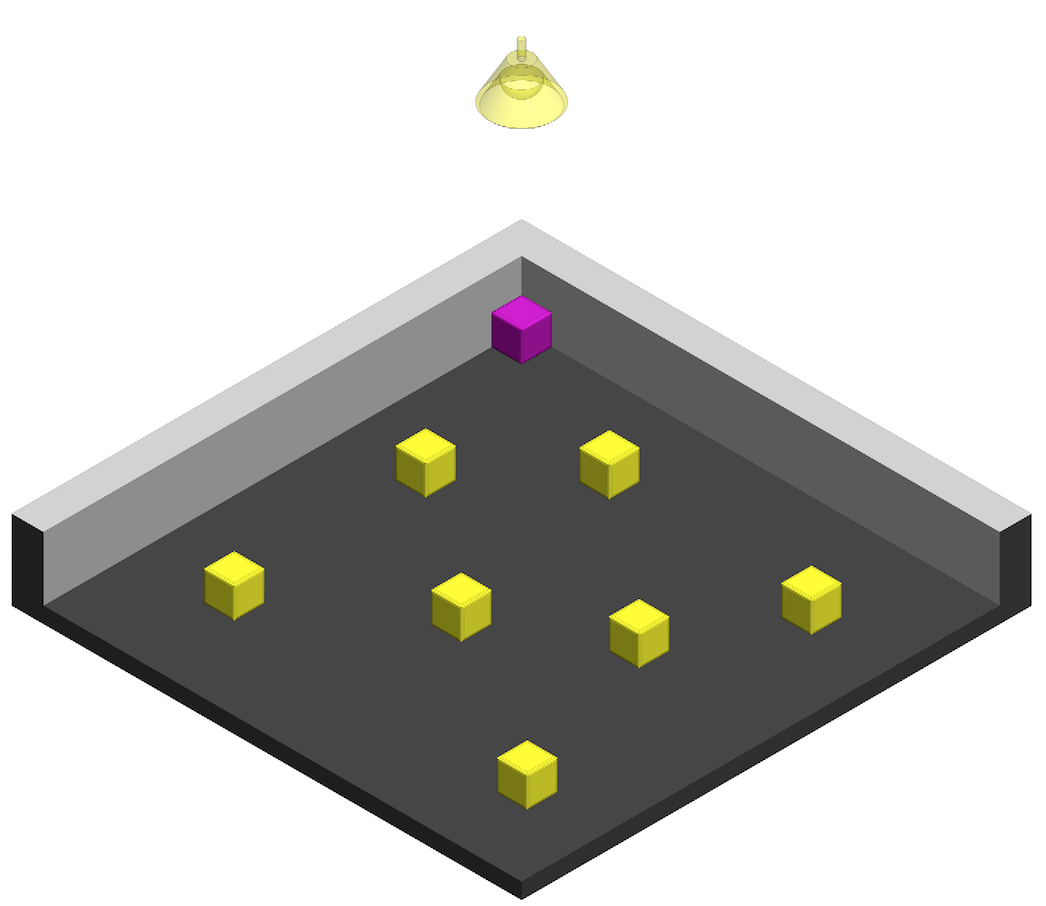
\includegraphics[width=0.9\linewidth]{figures/light_1.png}
%		\subcaption{} 
%	\end{subfigure}
%	\begin{subfigure}[b]{0.3\linewidth}
%		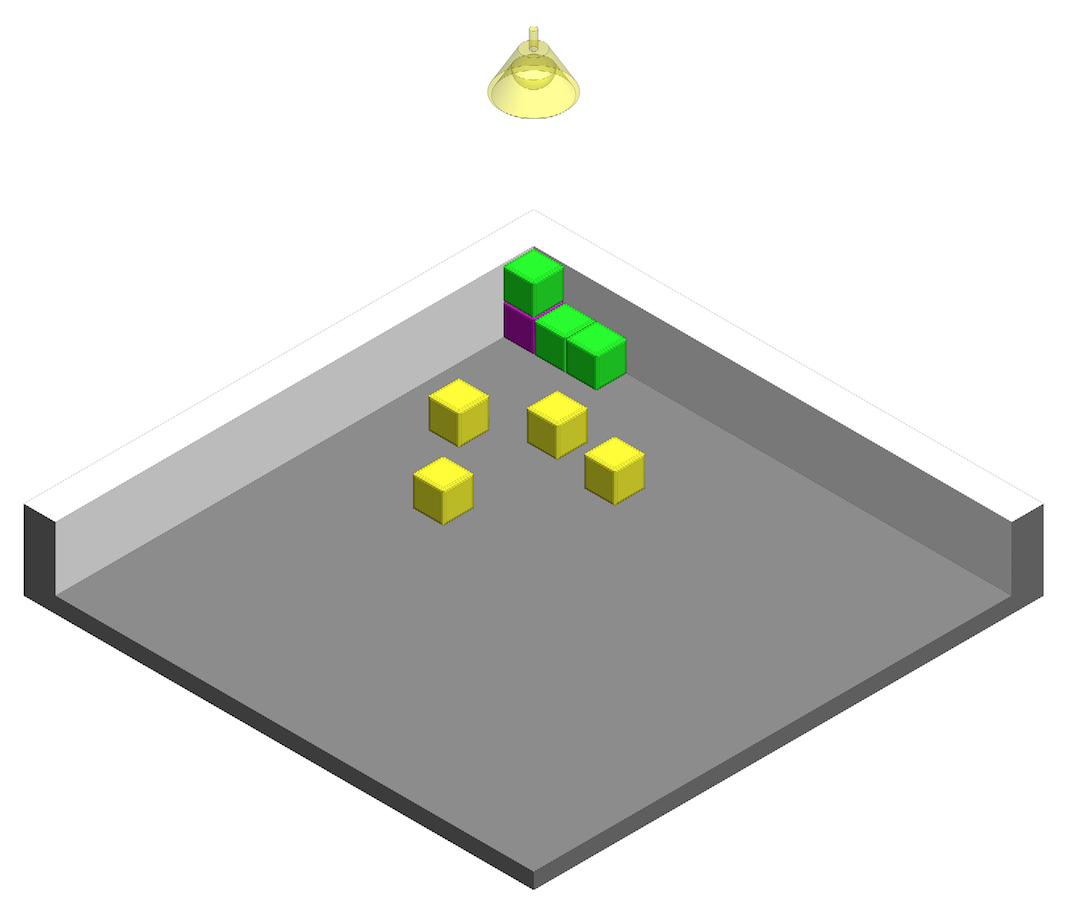
\includegraphics[width=0.9\linewidth]{figures/light_2.png}
%		\subcaption{} 
%	\end{subfigure}
%	\begin{subfigure}[b]{0.3\linewidth}
%		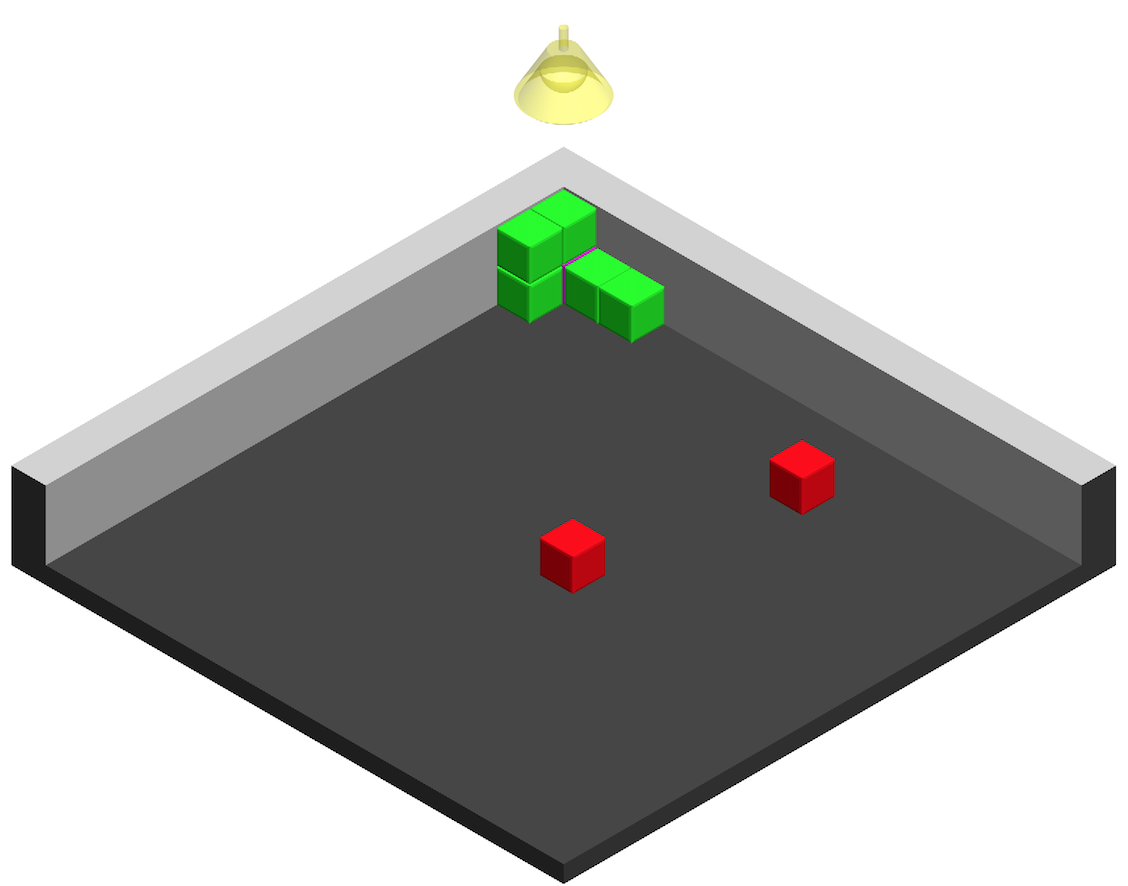
\includegraphics[width=0.9\linewidth]{figures/light_3.png}
%		\subcaption{} 
%	\end{subfigure}
%	
%	\caption{Three frames from an a illustration of the light-seeking experiment. One seed cube \emph{purple} is placed near the light, and the cubes in \emph{yellow} attempt to move towards the light. In the final frame, the modules which are in \emph{green} successfully reached the goal, while modules that are \emph{red} did not manage to join the target structure.}
%	
%	\label{fig:light}
%\end{figure}

\begin{algorithm}[htbp] 
	%\hrulefill
	\caption{Light guided aggregation Algorithm}
	\label{algorithmAggregate}
	\SetAlgoLined
%	\Kw{M-Blocks 3D}
%	initialization\;
	\While{Not connected to Goal Configuration}
	{
		Update State read sensors\;
		\uIf{Numer of Neighbors  = 0}
		{
			Roll in direction of the brightest face that isn't on top\;
		}
		\uElseIf{Neighbors = 1, but not at Goal}
		{
			Run algorithm to attempt to move towards light as a group\;
		}
		\uElseIf{Neighbors = 2, but not at Goal}
		{
			Disconnect from structure
		}
	}
	\caption{This algorithm attempts to drive a group of modules to form a single aggregated group based on following a light gradient.}
	
\end{algorithm}


%begin{figure}[h]  
%\centering
%
%\begin{subfigure}[b]{0.3\linewidth}
%	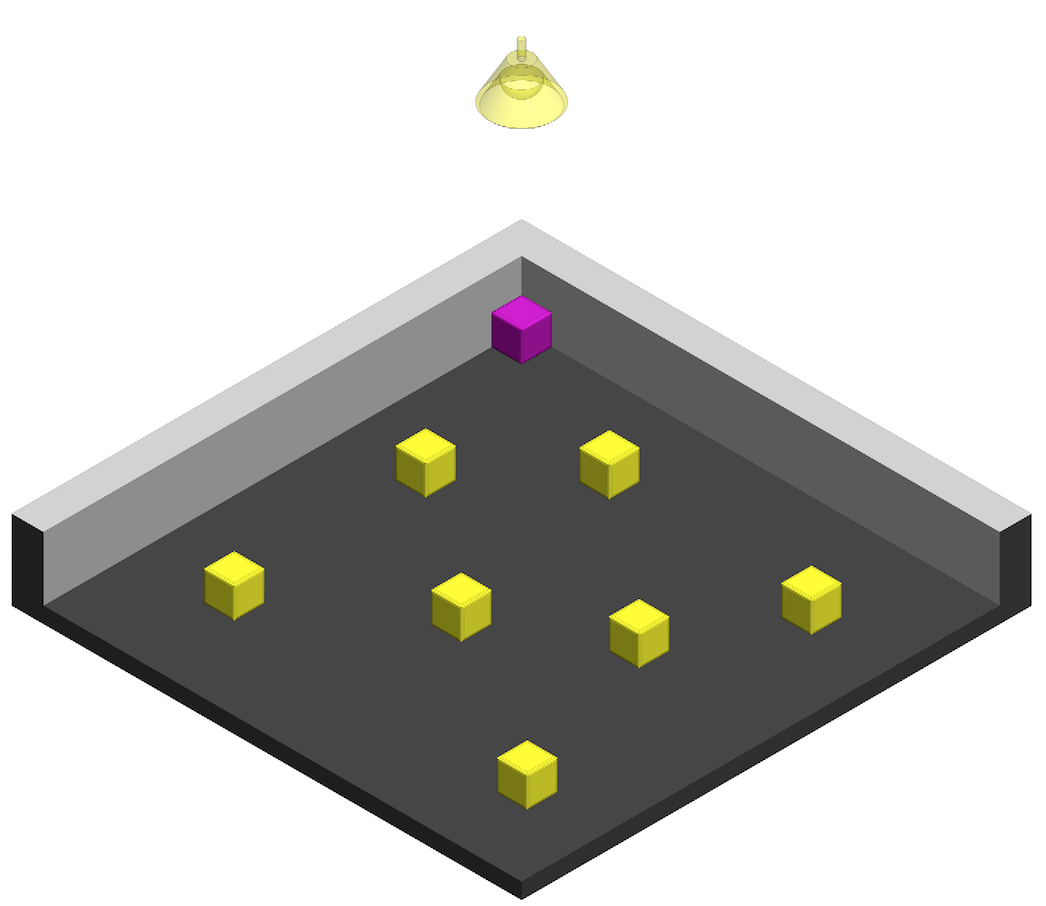
\includegraphics[width=0.9\linewidth]{figures/light_1.png}
%	\subcaption{} 
%\end{subfigure}
%\begin{subfigure}[b]{0.3\linewidth}
%	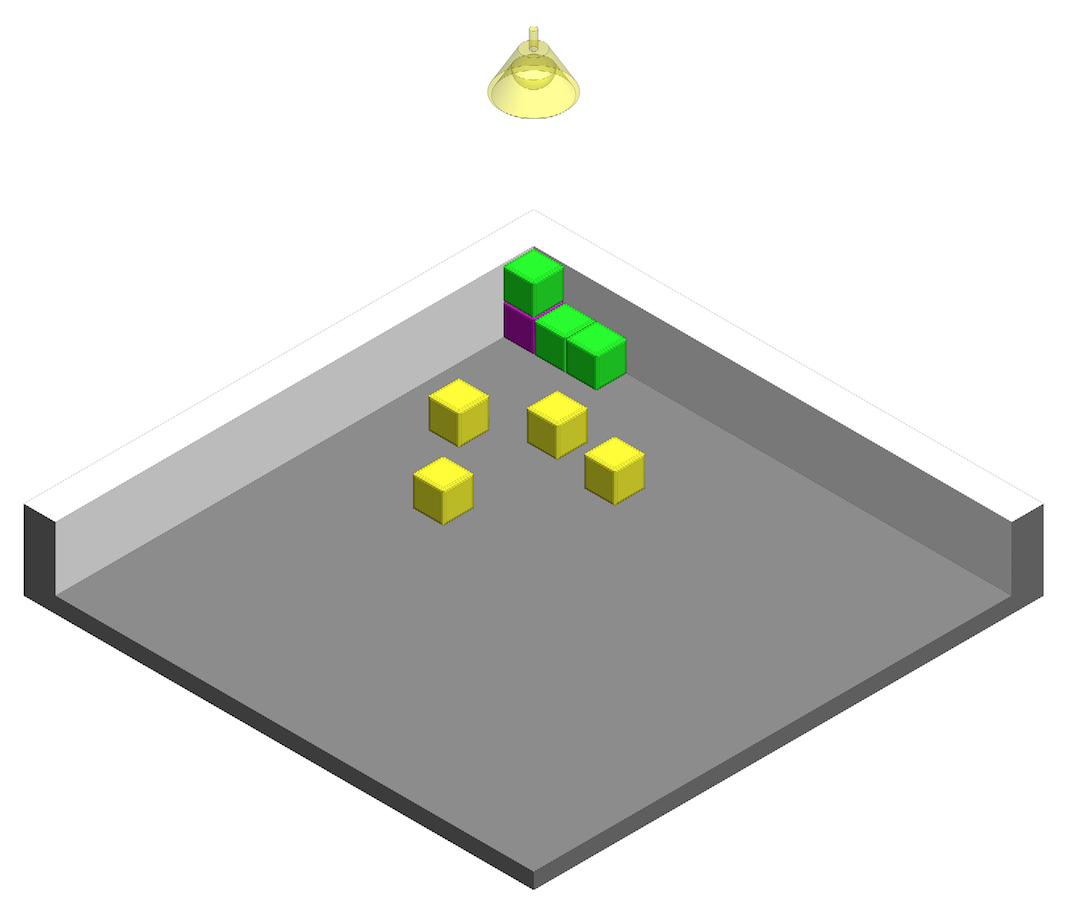
\includegraphics[width=0.9\linewidth]{figures/light_2.png}
%	\subcaption{} 
%\end{subfigure}
%\begin{subfigure}[b]{0.3\linewidth}
%	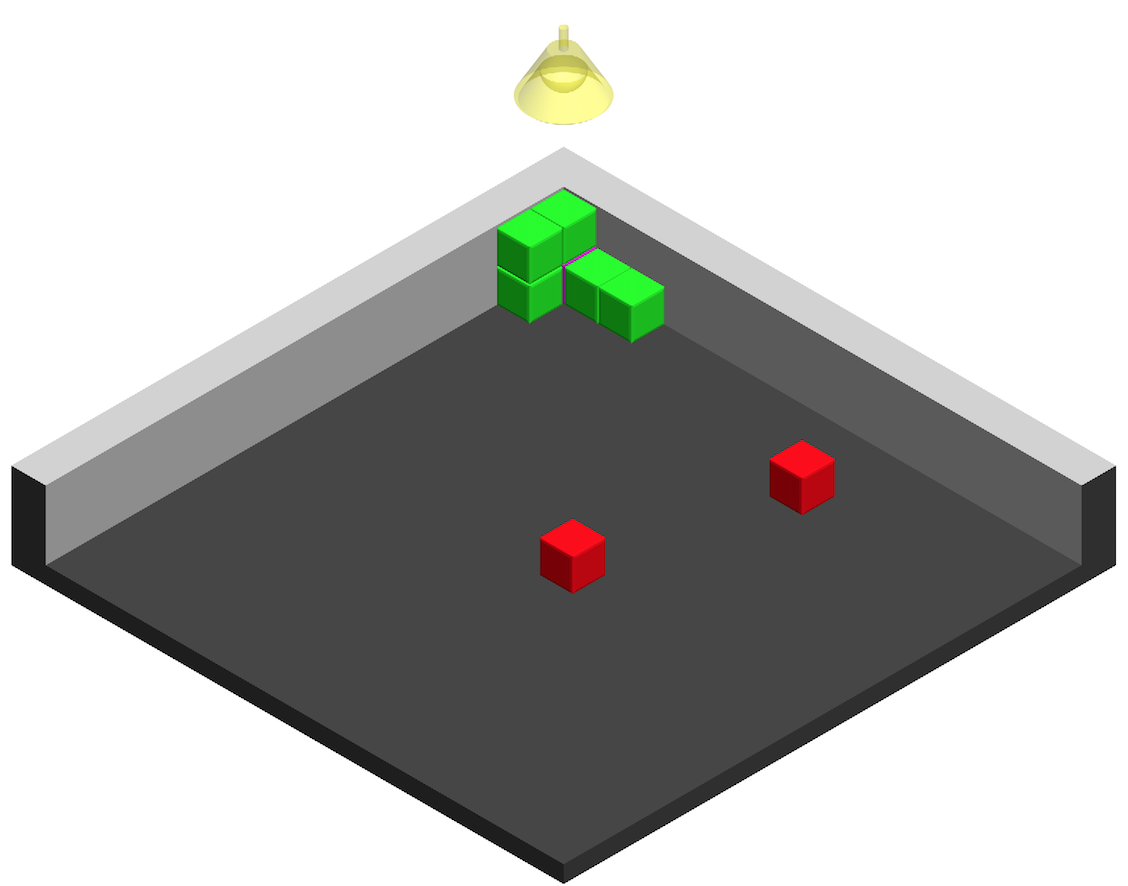
\includegraphics[width=0.9\linewidth]{figures/light_3.png}
%	\subcaption{} 
%\end{subfigure}
%
%\caption{Three frames from an a illustration of the light-seeking experiment. One seed cube \emph{purple} is placed near the light, and the cubes in \emph{yellow} attempt to move towards the light. In the final frame, the modules which are in \emph{green} successfully reached the goal, while modules that are \emph{red} did not manage to join the target structure.}
%
%\label{fig:light}
%\end{figure}

%
%\begin{figure}[h]  
%	\centering
%	\begin{subfigure}[b]{0.3\linewidth}
%		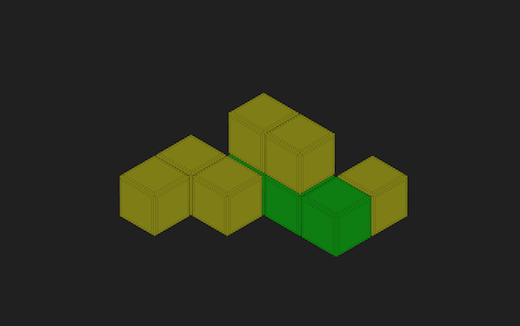
\includegraphics[width=0.9\linewidth]{figures/line_1.png}
%		\subcaption{} 
%	\end{subfigure}
%	\begin{subfigure}[b]{0.3\linewidth}
%		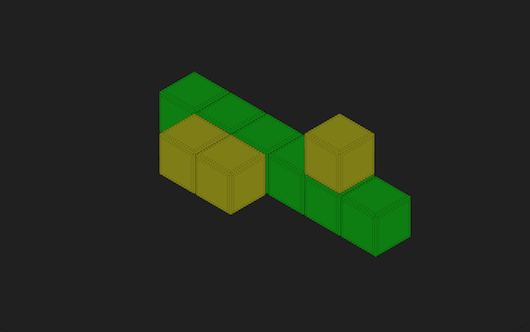
\includegraphics[width=0.9\linewidth]{figures/line_2.png}
%		\subcaption{} 
%	\end{subfigure}
%	\begin{subfigure}[b]{0.3\linewidth}
%		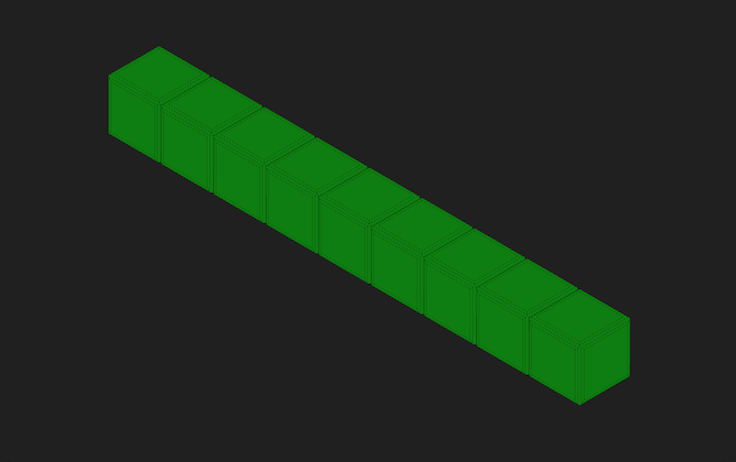
\includegraphics[width=0.9\linewidth]{figures/line_3.png}
%		\subcaption{} 
%	\end{subfigure}
%	
%	\caption{This experiment shows a random 3D configuration of M-Blocks reconfiguring into a line.}
%	
%	\label{fig:line}
%\end{figure}